\documentclass[10pt]{article}
\usepackage{latexsym}% Package loading the LaTeX symbol.
\usepackage{graphicx}% Package necessary to put graphics in your TeX document
\usepackage{setspace}% Package for changing space between the lines
\usepackage{fancyhdr}% Package for making the fancy headers with names of authors and title of paper
\usepackage{lscape}  % Package allowing to put your text in landscape
\usepackage{amsmath} % An extension package for LaTeX that provides various features to facilitate writing math formulas and to improve the typographical quality of their output
\usepackage{mathrsfs}
\usepackage{subfig,longtable,epsfig}
\usepackage{natbib}
\usepackage{epigraph}
\usepackage{rotating}
\usepackage{multirow}
\usepackage{rotfloat}
\usepackage{longtable}
\usepackage{booktabs}
\usepackage{threeparttable, textcomp}
\usepackage{enumerate}
\usepackage[colorlinks=true,pdfstartview=FitH,citecolor=blue,urlcolor=blue,linkcolor=blue]{hyperref} % Package allowing to make the hyperreferences in the text
\usepackage[latin1]{inputenc}
% entfernt: ,dvipdfm
\bibpunct{(}{)}{;}{a}{,}{,}
\def\BibTeX{{\rm B\kern-.05em{\sc i\kern-.025em b}\kern-.08em
    T\kern-.1667em\lower.7ex\hbox{E}\kern-.125emX}}
%%%%%%%%%%%%%%%%%%%%%%%%%%%%%%%%%%%%%%%%%%%%%%%%%%%%%%%%%%%%%%%%%%%%%%%%%%%%%%%%
% MARGINS
%%%%%%%%%%%%%%%%%%%%%%%%%%%%%%%%%%%%%%%%%%%%%%%%%%%%%%%%%%%%%%%%%%%%%%%%%%%%%%%%
\oddsidemargin 0cm \textwidth 17cm \textheight 23.00cm \topmargin
-1.5cm

\renewcommand{\baselinestretch}{2}
\begin{document}
\renewcommand{\thefootnote}{\fnsymbol{footnote}}

%\renewcommand{\thefootnote}{\ifcase\value{footnote}\or*\or
%**\or***\or****\or(\#)\or(\#\#)\or(\#\#\#)\or(\#\#\#\#)\or($\infty$)\fi}

\title{Do Media Data Help to Predict German Industrial Production?}
%\date{July 2014}

\author{Konstantin A. Kholodilin\footnotemark[1] \and Tobias Thomas\footnotemark[4] \and Dirk Ulbricht\footnotemark[3]}

\maketitle

\footnotetext[5]{An earlier version of this paper was presented at the 34th International Symposium on Forecasting in Rotterdam, from June 29 to July 2, 2014, at a research seminar of the Hamburg University on November 4, 2014, and at the 15th International Agenda Setting Conference held February 19-21, 2015in Vienna, Austria. We are thankful to participants of the conferences for their comments. The standard disclaimer applies.} 
\footnotetext[1]{Research associate, DIW Berlin, Mohrenstra\ss e 58, 10117 Berlin, Germany, \texttt{%
e-mail: \hspace{-0.1in}
\href{mailto:kkholodilin@diw.de}{kkholodilin@diw.de}}.}
\footnotetext[4]{Head of research, Media Tenor International, Alte Jonastra\ss e 48, 8640, Switzerland, and research affiliate,  D�sseldorf Institute for Competition Economics (DICE), Heinrich-Heine-Universit�t, Universit�tsstra�e 1, 40225 D�sseldorf, \texttt{%
e-mail: \hspace{-0.1in}
\href{mailto:t.thomas@mediatenor.com}{t.thomas@mediatenor.com}}.}  
\footnotetext[3]{Research associate, DIW Berlin, Mohrenstra\ss e 58, 10117 Berlin, Germany, \texttt{%
e-mail: \hspace{-0.1in}
\href{mailto:dulbricht@diw.de}{dulbricht@diw.de}}.}

\renewcommand{\thefootnote}{\arabic{footnote}} \setcounter{footnote}{0}

\setcounter{page}{1} \pagenumbering{Roman}

\begin{abstract}
In an uncertain world, decisions by market participants are based on expectations. Therefore, sentiment indicators reflecting expectations have proven track record at predicting economic variables. However, survey respondents largely perceive the world through media reports. Here, we want to make use of that. We employ a rich data set provided by Media Tenor International, based on sentiment analysis of opinion-leading media in Germany from 2001 to 2014, transformed into several monthly indices. German industrial production is predicted in a real-time out-of-sample forecasting experiment and media indices are compared to a huge set of alternative indicators. Media data turn out to be valuable for 10 to 12 months horizon forecasts. This holds in the period during and after the financial crisis when many models fail.
\\ \\
\textbf{Keywords}: media data, German industrial production, forecast breakdown, real-time experiment, model confidence set.
\\
\textbf{JEL classification}: C10; C52; C53; E32. 
\end{abstract}

%%%%%%%%%%%%%%%%%%%%%%%%%%%%%%%%%%%%%%%%%%%%%%%%%%%%%%%%%%%%%%%%%%%%
\newpage
\tableofcontents

\newpage
\listoftables \listoffigures

\newpage
\setcounter{page}{1} \pagenumbering{arabic}

%%%%%%%%%%%%%%%%%%%%%%%%%%%%%%%%%%%%%%%%%%%%%%%%%%%%%%%%%%%%%%%%%%%%
\newpage

\section{Introduction}

Typically, the data on gross domestic product (GDP) are available on a quarterly basis. In addition, they are published half a quarter following the end of the reference quarter. Therefore, in order to gain quick insight into the current economic situation, a monthly series of industrial production is used. It is considered as a key monthly indicator for business activity.
This is especially true in the case of Germany. Although the share of industrial
production has been shrinking since the 1980s, it remains relatively high when compared to other OECD and, especially, other EU member countries.%
\footnote{According to the OECD Factbook 2011: Economic, Environmental and Social
Statistics, in 2010, the percentage of total value added in industry
(including energy) was 24\% in Germany, 19\% in the EU,
and 21\% in the OECD countries.} 
Furthermore, the European Commission plans to raise the contribution of industry to GDP to as much as 20\% by 2020 (\citealp{european_commission_industrialization_2014}) in order to increase the competitiveness of the EU.
Moreover, industrial production contributes substantially to the business cycle dynamics.

Consequently, there have been many attempts to improve the forecast accuracy
of this variable.%
\footnote{See, for example, \cite{kholodilin_siliverstovs_2006}, \cite{robinzonov2009freedom} or \cite{drechsel2012performance}.} Most of these studies employ hard economic indicators, such as interest rates, manufacturing orders, etc. There are also several studies using soft data, such as business surveys, like the ifo or ZEW indicator (see, for example, \citealp{abberger2006einige} or \citealp{hufner2002prognosegehalt}).
It is demonstrated that due to their forward-looking nature, the soft data are well-suited for forecasting industrial production. The underlying idea of this approach is to employ a measure of the intentions or the expectations of the managers or analysts, respectively. The main advantages of these indicators are their high frequency, timeliness, and the fact that they are never subject to revisions, unlike many other statistical indicators. 

While in classical economics the \textit{homo oeconomicus} is omniscient and decides independently, with his decisions leading to efficient outcomes at the market level, \citet{keynes1937general} underlines the role of uncertainty concerning decisions and behavior as well as the related (suboptimal) outcomes at the macro level, just as \citet{von1992pretence} points to the pretense of knowledge. Similarly, \citet{simon1957models} as well as \cite{Kahneman_Tversky_1979} show that actual human behavior clearly deviates from the behavior predicted by standard economic models. Due to their limited information processing capacity, individuals use subjective models for the perception of reality. If these models are shared because of common cultural background and experience, in accordance with \citet{denzau1994shared}, one can speak of shared mental models. In media societies, media reporting forms relevant parts of those shared mental models not only because investors, consumers, politicians, and voters receive lots of information via the media, but because additional information perceived directly is interpreted on the basis of the frame determined by the media reporting. Therefore, what is on the agenda (``agenda setting'') and what is not (``agenda cutting'') becomes highly relevant, as well as the way in which these things are described in the media, such as with a positive, negative or neutral tone. At least in part, individuals decide and behave  based on the information they receive from the media. This is also important in the context of business surveys, as respondents interpret their own economic situation and build their expectations within the frame set by the media.

A growing literature employs media data to explain economic sentiment. For instance, \cite{Goidel_Langley_1995} as well as \cite{Doms_et_al2004} show an impact of media reporting on consumer climate. For \cite{Nadeau_et_al_2000} and \cite{Soroka_2006} the assessment of the state of the economy depends at least in parts on media reports. In their comprehensive contribution \cite{lamla2012} analyze the role of media reporting for inflation forecasts of households and professional forecasters.%

The literature can be split into two main streams. The first one counts the number of times a single word or a group of words, which can be associated with a
certain event, occur in the media. The second strand of literature
captures content expressed in the media. 

Most economic analyses using media focus on the United States.  Using word counts, \emph{The Economist} newspaper introduced the R-word index, which is a proxy for the US business cycle. It counts how many articles in \emph{The Washington Post} and \emph{The New York Times} use the word \textquotedblleft{}recession\textquotedblright{} in a quarter. This simple indicator was expanded by \citet{Doms_et_al2004}, who count the number of articles in 30 American newspapers that contain 9 keywords or expressions in the title or the first paragraph of an article and use this statistic to forecast US private consumption. 

Beyond simple word counts, content analysis focuses on the underlying sentiment expressed in media reports using both automated methods and human analysts to evaluate the news. \citet{Tetlock2007}
evaluates the sentiment of \emph{Wall Street Journal} articles, while  \citet{Uhl2010, Uhl2012} uses sentiment data of newspaper and TV-news, provided by Media Tenor International, to forecast US private consumption. 

\citet{Bordino_et_al2011} use the number of queries of listed companies in the US search engine Yahoo! as a predictor for stock market volumes. Using the number of queries in Google, \citet{Kholodilin_et_al_2010} try to improve forecasts of US private consumption. \citet{Bollen_et_al2011}
employ the OpinionFinder software to analyze Twitter tweeds automatically with the aim of forecasting stock prices.


For Germany, the R-word index was adopted HypoVereinsbank, which counted the word \textit{Rezession} (``recession" in German) in articles published in the \emph{Frankfurter Allgemeine Zeitung}, \emph{Handelsblatt}, and \emph{WirtschaftsWoche}; but publication of the index was quickly given up.%
\footnote{The German R-word index was reported in the mass media several times in the early 2000s but no instances were were identified after July 5 2001.}  \citet{Grossarth_et_al2008} revived the index for their study, but at that time the Great Recession period could not be considered. Their study uses media indices to predict German industrial production, contrasting the R-word index for Germany and a Media Tenor International index to predict growth rates of industrial production and of recession probabilities. For both indices the results are rather mixed. Other media studies include \citet{Iselin_Siliverstovs2013}, who use the R-word index to forecast the growth rates of real GDP in Germany and Switzerland. While media indicators are helpful for Switzerland, it is not the case for Germany. \citet{Ammann_et_al2011} compute the number of mentions of a lexicon of 236 words in the online archive of \emph{Handelsblatt} with the aim of predicting yields of the German stock market DAX index. They show that newspaper content is a valuable predictor of future DAX returns.

Here, we test the predictive content of media indicators performing a pseudo-out-of-sample forecast experiment. Since we want to compare the performance of the media indicators to that of an as complete as possible set of rival indicators, we collect and update the database of \citet{drechsel2012performance}, which set a standard in this respect. 

This paper makes five contributions: First, unlike \citet{Grossarth_et_al2008} who use a single aggregate Media Tenor International business conditions index, we employ 16 more indicators that differ in their time perspective (present, future, and climate), their underlying topic (government budget, monetary policy, labor market, and business cycle, taxation), and the region it is reported about (Germany and the rest of the world, ROW). Second, in contrast to \citet{Grossarth_et_al2008}, we use monthly instead of quarterly data. Third, in contrast to \citet{drechsel2012performance} and \citet{Grossarth_et_al2008} we take advantage of real-time data provided by the Deutsche Bundesbank for the industrial production as well as for other crucial variables such as inflation. This is particularly important in this context as one of the great benefits of media data is that they do not need to be revised \emph{ex post}. Fourth, we test media-based models against \textit{data snooping} using Model Confidence Set approach (\citealp{hansen2011model}). Fifth, we separately test the media indicators' relative performance over a period when forecasting becomes particularly difficult. To the best of our knowledge we are the first to identify such a period using the concept of forecast breakdowns introduced by \citet{giacomini2009detecting}. Finally, we employ the same concept to compare the reliability of different indicators.

Summing up, we find that media indicators based on news that are related to future events are very useful for predicting 10 to 12 months ahead. This is also true during periods when forecasting becomes harder. %We show that the period does not coincide with the recession period dated by the Economic Cycle Research Institute (ECRI). 
 
This paper is structured as follows. The second section presents the empirical approach  and the third section describes the forecast accuracy tests employed. In section four the data used in the analysis are presented, in section five the results are discussed and the last section concludes.

\section{Empirical approach}

We follow the approach of existing studies that concentrate on the comparison of single models that include one different alternative indicator at a time in a horse race with respect to forecast accuracy.  

Due to the different release lags of indicators such as macroeconomic
or survey indicators, data unbalancedness often emerges at the end
of multivariate samples. This phenomenon is sometimes referred to as
the ragged-edge of the data. In order to account for this we adapt
the basic empirical setup for individual models from \citet{drechsel2012performance} that
explicitly addresses this issue. The estimation equation for the individual
models is given as: 
\begin{equation}
y_{t+h}^{h}=\alpha+\sum_{p=\underline{p}}^{P}\beta_{p}y_{t-p}+\sum_{q=\underline{q}}^{Q}\gamma_{q}x_{t-q}+\epsilon_{t+h}^{h}\label{eq:individual models}
\end{equation}
where $y_{t+h}^{h}$ is the annualized growth rate of industrial production at time $t$
over the next $h$ months, $y_{t+h}=1200/h\times\ln(\mbox{IP}_{t}/\mbox{IP}_{t-h})$.
The growth rate of industrial production in levels, $\mbox{IP}_{t}$, is
defined as $y_{t}=\Delta\ln \mbox{IP}_{t}$; $x_{t}$ is a candidate predictor;
$\epsilon_{t+h}^{h}$ is an error term; and $\alpha$, $\beta$, and
$\gamma$ are regression coefficients. The timely availability of indicator variable can
be taken account of by $\underline{p}$ and $\underline{q}$. German industrial production
is available only with a time lag of $\underline{p}=3$ months. The publication lags of the candidate regressors vary from $\underline{q}=0$, mostly for financial and media data, up to $\underline{q}=2$ months. The lag length is optimized using the Akaike information criterion. First, $P$ is estimated. Then, holding $P$ fixed, $Q$ is estimated.

Forecasts for 1 to 12 months horizons are computed in a pseudo-out-of-sample real-time setup:
\begin{itemize}
\item The first forecast is made based on the information set as it has been available in 2005:12.
\item Each iteration, the information set is extended by one month, that is, in the second iteration, data are used as they have been available in 2006:01, in the third iteration data available in 2006:02 are used, and so on. 
\item For each horizon, individual models are estimated and forecasts are made. 
\item Each iteration, the lag-length are optimized and the model is
updated.
\item All real indicators are deflated using consumer price index as it has been available at the point in time the forecast is made. 
\item The estimations are based on a rolling window of 60 months. Employing
rolling windows is a method of dealing with slowly moving non-stationarities, see, e.g., \citet{pesaran2004costly}. Furthermore, it is required for the Model Confidence Set (MCS) test, see \citet{hansen2011model}.
\item The last one is based on the information set available in 2014:11 for $h=1$, respectively 2013:11 for $h=12$.
\end{itemize}

After having completed the estimation and forecasting exercise, the forecasts are used to compute the forecast errors based on the data as they have been available 2015:02 (current vintage data). 
%\subsection{Data\label{sec:Data}}

\section{Forecast accuracy tests}

To compare the usefulness of media indicators relative to rival indicators for predicting German industrial production we need to evaluate the forecast performance of competing models. Thereby, we recur to simple forecast accuracy measures, pairwise and multiple statistical tests, and a test for forecast breakdowns.

\subsection{Simple measures}

In the following, we concentrate on one of the standard loss functions adopted in
the forecasting literature: the squared forecast error, $L_{it}=e_{it}^{2}$.
Let $e_{it}=y_{t}-\hat{y}_{it}$  be the forecast error of
model $i$  in period $t$, where $y_{t}$ is the realization of
the target variable and $\hat{y}_{it}$ is the value forecast
by model $i$. Usually, the forecast performance of alternative models
is compared using the mean squared forecast error (MSFE) defined as 

\begin{equation}
MSFE_{i}=\frac{\sum_{t=T_E+1}^{T_E+T_F}e_{it}^{2}}{T_F},
\end{equation}
where $T_E$ is the length of estimation period, and $T_F$ is the number of forecasts. However, by making use of squared
forecast errors the $MSFE_{i}$ tends to overly emphasize differences
between models. Thus, we will concentrate on the root mean squared
forecast error, $RMSFE_{i}$. Moreover, for pairwise comparisons we employ the
Theil's $U$ defined as
\begin{equation}
TU_{i}=\frac{RMSFE_{i}}{RMSFE_{0}}
\end{equation}
measuring the relative performance of model $i$, $RMSFE_i$, with respect to that of
a benchmark model, $RMSFE_0$. A value exceeding one implies that the alternative model $i$ is less accurate than the benchmark, whereas a value lower than one implies that it is more accurate. 


\subsection{Tests}

\subsubsection{Pairwise tests}

Our aim is to test if media data contain any valuable information for forecasting purposes. A minimum requirement is that media data improve upon the forecasts obtained using a simple autoregressive (AR) model. This involves pairwise comparisons of the AR model and alternative models consisting of the AR model augmented with one additional explanatory variable at a time.
Let the loss difference be $d_{it}=L_{0t}-L_{it}$.
The starting point for pairwise forecast comparisons of a benchmark
model, $0$, and an alternative model $i$ is the \citet{diebold1995comparing} test statistic
defined as: 
\begin{equation}
DM=\frac{\overline{d}_{i}}{\hat{V}(\overline{d}_{i})}
\end{equation}
where $\overline{d}_{i}$ and $\hat{V}(\overline{d}_{i})$ are the estimated mean and long-run variance of $d_{it}$, respectively.
The null hypothesis of the test is

\begin{eqnarray}
H_{0}: & E(d_{it})=0,\label{eq:dm null}
\end{eqnarray}
that is, that the two models perform equally well.

By construction, the AR is nested in the augmented model. Under the
null hypothesis, the additional variables are useless and their regression coefficients
are zero. However, estimating additional variables introduces noise
into the forecasts of the alternative model. Consequently, under the
null, the forecast accuracy of the smaller benchmark is higher than that of
the larger alternative model. Thus, in the context
of nested models, the DM statistic has lower power and size. Therefore,
we apply the modified test statistic of \cite{Clark_West_2007}, which
involves an adjustment term to improve upon the DM statistic when nested models are compared:
\begin{equation}
CW=\frac{\overline{d}_{i}-\overline{a}_{i}}{\hat{V}(\overline{d}_{i}-\overline{a}_{i})},
\end{equation}
where $\overline{a}_{i}=\frac{1}{T_F}\sum_{t=T_E+1}^{T_E+T_F}(\hat{y}_{0t}-\hat{y}_{it})^{2}$.


\subsubsection{Multiple tests}

\cite{white2000reality} points out that, even when no exploitable forecasting
relation exists, looking hard enough at a given set of data will often reveal one or more forecasting models that appear to be good, but are, in fact, useless. In particular, sequential testing a number of models by comparing two of them at a time invalidates standard critical values and might result in
\textit{data snooping}. In much of economic time series analysis this is aggravated
by the fact that typically there is only a limited number of observations
available. To overcome this problem \cite{white2000reality}, proposes a reality
check test (RC-test) for data snooping. It compares the whole set of $m$ rival models at a time to the benchmark. The null hypothesis is that none of the rival models is inferior to the benchmark:
\begin{eqnarray}
H_{0}: & E(d_{it})\leq0 & \forall i=1,\ldots,m.\label{eq:white null}
\end{eqnarray}

It is rejected when at least one of the rivals yields significantly better forecasts. The expected loss differential can be consistently estimated using the sample mean, $\overline{d}_{i}$. White proposes the sample mean statistic
\begin{equation}
RC=\max_{k=1,...,m}T^{1/2}_F\overline{d}_{k}.
\end{equation}

This approach has subsequently been refined by \cite{Hansen_2005}. He shows
that the test statistic proposed by White is very conservative, if
the set of rival models contains very poorly performing models, and
proposes a refinement consisting of a studentized version of the RC-test
that is known as the test for superior predictive ability (SPA). 

However, selecting the benchmark independently of the data introduces
the problem of \textit{multiple comparisons} \textit{with control}.
To overcome this \citet{hansen2011model} propose the model confidence set (MCS) approach. This approach consists in looking for a set of best models, $\mathcal{M}^{*}$, such that, given
the set of all forecasting models, $\mathcal{M}_{0}$, the MCS identifies the set of forecasting models that cannot be rejected as statistically inferior at a certain level of confidence:

\begin{equation}
\mathcal{M}^*=\left\{ i\in\mathcal{M}_{0}:\,\mu_{ij}\leq0\,\mbox{ for all }\, j\in\mathcal{M}_{0}\right\} 
\end{equation}
where $\mu_{ij}=E(d_{ij})$ is the expected loss differential $d_{ij}=L_{it}-L_{jt}$
based on one-by-one comparisons of all models.%
\footnote{Here again, we choose the squared forecast error as loss.%
} The MCS is implemented using the following steps, where initially $\mathcal{M}$
is set $\mathcal{M}=\mathcal{M}_{0}$:
\begin{enumerate}
\item The null of equal predictive accuracy (EPA), $H_{0,\mathcal{M}}:\,\mu_{ij}\leq0\,  \forall i,j$
is tested at significance level $\alpha$. \label{enu:Beginning-with-the}
\item If the null is rejected, the worst performing model is eliminated from
$\mathcal{M}$.
\item The procedure is repeated until the null cannot be rejected. The
set $\mathcal{\widehat{M}}_{1-\alpha}^{\text{*}}$ with the remaining
models is defined as the MCS.
\end{enumerate}
In order to test the null hypothesis in step \ref{enu:Beginning-with-the} we
apply the $T_{max,\mathcal{M}}$ statistic.%
\footnote{\citet{hansen2011model} propose an alternative test statisitics, $T_{R,\mathcal{M}}$.
Here, we only report the results for $T_{\max,\mathcal{M}}$ statistic
 as it yielded the most conservative results, that is, the smallest
confidence sets.%
} Let $\overline{d}_{ij}\equiv T_F^{-1}\sum_{t=T_E+1}^{T_E+T_F}{d}_{ij}$ be the relative sample loss between the $i$th and the $j$th models. Then let $\overline{d}_{i\cdot}$ be the loss of the $i$th model relative to the average across models in $\mathcal{M}$, $\overline{d}_{i\cdot}\equiv m^{-1}\sum_{j\in\mathcal{M}}\overline{d}_{ij}$, where the models in $\mathcal{M}$ are again indexed by $i=1,\ldots,m$. Then,
the $t$-statistic is defined as:

\begin{equation}
t_{i\text{\ensuremath{\cdot}}}=\frac{\overline{d}_{i\cdot}}{\sqrt{\widehat{V}(\overline{d}_{i\cdot})}}
\end{equation}
where $\widehat{V}(\overline{d}_{i\cdot})$ is an estimate of $V(\overline{d}_{i\cdot})$.
The $t$-statistic can be associated with the null $H_{i\cdot}:\mu_{i\cdot}=0$,
where $\mu_{i\cdot}=\textrm{E}(\bar{d}_{i\cdot})$. \citet{hansen2011model} show
that the hypothesis $H_{0,\mathcal{M}}$ is equivalent to $\{H_{i\cdot}\mbox{ for all  }i\in\mathcal{M}\}$
such that $\{\mu_{i\cdot}\leq0\mbox{ for all }i\in\mathcal{M}\}$.
Thus, the null hypothesis $H_{0,\mathcal{M}}$ can be tested using
the statistic:

\begin{equation}
T_{\max,\mathcal{M}}=\max_{i\in\mathcal{M}}t_{i\cdot}
\end{equation}
The asymptotic distribution of $T_{\max,\mathcal{M}}$ is nonstandard
as it depends on nuisance parameters. However, it can be estimated
using bootstrap methods. 

In the best of all cases, the MCS contains only one model. However,
if the data are uninformative, the MCS contains several models or
even all models in $\mathcal{M}_{0}$. As a useful feature,
the MCS procedure yields a $p$-values for all models under consideration
where a small $p$-value indicates that the corresponding model is unlikely to enter the set
of superior models, $\mathcal{M}^{*}$(for details, see \citealp{hansen2011model}).

\subsection{Forecast breakdowns}

Reliability of models is crucial for forecasters. However, models may become unstable over time due to instabilities in the economy. Thus, forecasting performance depends on the success of the model at adapting to changes. 
%A common way to test for the adaptability is to evaluate forecast performance during instable times, like recessions as exogenously dated by some institution (see, e.g., \citealp{stock2003did} or \citealp{drechsel2012performance}). However, recessions and phases of poor forecasting performance need not coincide. In the case at hand, industrial production dropped sharpely only at the end of the recession (see Section \ref{sec: results} below) which raises doubts about this approach.  Thus, to test for the adaptability we define an instable period relying on the concept of forecast breakdowns proposed by \citet{giacomini2009detecting}. Their approach
\citet{giacomini2009detecting} introduce an approach to test whether the model's future performance is consistent with what is expected on the basis of its past performance. They define a forecast breakdown as a situation, in which the out-of-sample performance of a forecast model, judged by some loss function, is significantly worse than its in-sample performance. Their test is based on the intuition that, in the absence of a forecast breakdown, the difference between expected out-of-sample and in-sample performances should be close to zero.

The approach has two major advantages: First, in contrast to the literature
concentrating on structural breaks, such as, \citet{bai2003computation}, the forecast breakdown
test allows for model misspecification. Second, the test is applicable
in cases of instabilities in the data generating process of unknown
form. 

Let $y_{t+h}$ be a sequence of $h$\textminus{}step-ahead forecasts
from an out-of-sample forecast experiment, which involves dividing
the sample of size $T$ into an in-sample window of size $T_E$ and
an out-of-sample window of size $T_F^h=T-T_E-h+1$.
A surprise loss at time $t+h$ is defined as the difference between
the out-of-sample loss at time $t+h$ and the average in-sample loss: 

\begin{eqnarray}
SL_{t+h}=L_{t+h}-\overline{L}_{t}, &\mbox{for} & t=T_E,\ldots,T\text{\textminus}h\label{eq:surprise loss}
\end{eqnarray}
where $\overline{L}_{t}$ is the average in-sample loss computed over
the in-sample window. If a forecast is reliable, this mean should
be close to zero. Thus, the null is defined as 
\begin{eqnarray}
H_{0}: & E\Bigg(T_F^{-1}\sum_{t=T_E}^{T-h}SL_{t+h}\Bigg) = 0,\label{eq:fb test statistic}
\end{eqnarray}
where $T_F^{-1}\sum_{t=T_E}^{T-h}SL_{t+h}$ is the out-of-sample mean
of the surprise losses. The test statistic is then defined as 
\begin{equation}
t_{T_E,T_F,h}=T_F^{1/2}\overline{SL}_{T_E,T_F}/\hat{\sigma}_{T_E,T_F},
\end{equation}
where $\hat{\sigma}_{T_E,T_F}^{2}$ is an asymptotic variance estimator.

%\section{Empirical approach and data\label{sec:Empirical-approach-and}}


\section{The data}

Our contribution is based on the assessment by Media Tenor International (MTI), the Swiss-based media analysis institute, of the content of opinion-leading media in Germany, including five TV news programs, two weekly magazines, and one daily tabloid newspaper. News items only referring to the state of the economy in the media set were analyzed over the period from January 1, 2000 through March 31, 2014. Hence, the analyzed data set  can be seen as a subset of a much bigger data set including news items on all possible protagonists, such as persons (politicians, entrepreneurs, managers, celebrities, etc.) and institutions (political parties, companies, football clubs, etc.).  Each of these news items was analyzed with regard to the topic mentioned (unemployment, inflation, etc.), the region of reference (for example, Germany, EU, USA, UK, BRIC, worldwide), the time reference (past, present, and future), the source of information (journalist, politician, expert, etc.), as well as with regard to the tone of the information (negative, positive or neutral).%
\footnote{Media Tenor International employs professional coders to carry out media-analysis. Only coders that achieved a minimum reliability of 0.85 are cleared for coding. That means that the coding of these coders deviate at most by 0.15 from the trainers' master-versions. The reliability of the coding is checked on an ongoing basis, both with quarterly standard tests and random spot checks. For each month and coder, three analyzed reports are selected randomly and checked. Coders scoring lower than 0.80 are removed from the coding process. In none of the months the mean deviation among all coders was above 0.15.} 
Overall 80,675 news items about the state of the economy are included in the analysis. For a description of the analyzed media set see Table \ref{tab:Analyzed-Media-Set}. Of all the topics only government budget, monetary policy, labor market, business cycle, and taxation contain enough observations to compute subindices with a complete set of monthly observations. Table \ref{tab:contingency} is a contingency table of these topics. It reports the number of observations of the topics in temporal (present, past, and future) and spatial dimensions (Germany vs. the rest of the world). 

\begin{center}
Table {[}\ref{tab:Analyzed-Media-Set}{]}
about here
\par\end{center}
 
We computed 17 MTI indices using different (sub)samples of the news data. We distinguish between two types of indices depending on the way they are constructed.

The first type is the difference between the percentage share of the
positive ratings and that of the negative ratings:

\begin{equation}
B_{i,j,t}=100\times\frac{A_{i,j,t}^{+}-A_{i,j,t}^{-}}{A_{i,j,t}^{+}+A_{i,j,t}^{-}+A_{i,j,t}^{0}}
\end{equation}
where $A_{i,j,t}^{+}$ is the number of positive ratings of media reports
about events happening in time $i$ in the country $j$, published
in the period $t$, $A_{i,j,t}^{-}$ is the number of negative ratings,
and $A_{i,j,t}^{0}$ is the number of neutral ratings. The index varies
between $-100$ (all reports are negatively rated) and 100 (all reports
are positively rated).

The second type uses the indices of the present and the future sentiment to construct a so-called \textbf{media climate index} analogous to the ifo business climate index: 
\begin{equation}
MCI=\sqrt{(B^P_{j,t}+100)(B^F_{j,t}+100)}\label{eq:MCI}
\end{equation}
where $B^P_{j,t}$ is the present sentiment index and $B^F_{j,t}$
is the future sentiment index. By construction, the MCI can take values
between 0 indicating extremely bad media climate and 200 pointing
to an excellent media climate.

Based on these two types, we distinguish between four groups of MTI indicators:
\begin{enumerate}
\item The first set of indicators differ only in the time reference of the respective databases. MT.all uses all the data with all time references (past, present, and future). MT.present and MT.future are based on the data with the time references present and future, correspondingly. Finally, MT.climate, is computed based on the items with present and future reference as in equation (\ref{eq:MCI}). 
\item The second group is the same as the first. However, it exclusively uses data with a reference to Germany. The indices are labeled with "de".
\item The second group of indicators only uses data related to specific topics: The government budget (MT.budget), monetary issues (MT.monetary), the labor market (MT.labor), the business cycle (MT.cycle), and taxation (MT.taxation). The selection of subsets is restricted by data availability. The more specialized the topic, the fewer observations available.  
 \item The fourth group is the same as the third, however, it exclusively uses data with a reference to Germany. The indices are again labeled with ``de".%
\footnote{As the number of observations for MT.de.monetary would have been too small, it was not constructed.}
\end{enumerate}

Table \ref{tab:Media-indices,-descriptive} shows the mean and the median of the media indices. Except for MT.climate and MT.de.climate all indices have a negative mean. This is in line with the literature (see, for example, \citealp{brettschneider2000reality}) that finds that negative news dominates the media. Moreover, the standard deviations of of some subindices, particulary MT.cycle and MT.de.cycle are very high when compared to MT.all, which is based on the whole data set. Figure \ref{fig:MT-indices-all} shows the indices with a regional reference to all countries (groups 1 and 3) and Figure \ref{fig:MT-indices-de} show the indices with a reference to only Germany (groups 2 and 4). 

In addition to the media indicators, we collected variables from the database used
in \citet{drechsel2012performance}. This is a large data set comprising financial
indicators, survey indices, prices and wages, indicators of the real economy,
and composite indicators. For details see Table \ref{tab:indicators} and \citet{drechsel2012performance}.%
\footnote{Some of their variables are missing in our data set. We could not construct five spread series involving corporate rates computed by Merryl Lynch and the
early bird indicator of the Commerzbank as we did not obtain the data.
Furthermore, we only obtained very short series for the purchasing
manager index of Markit. Finally, we did not include monetary aggregates
as, since the introduction of the euro, no country-specific monetary aggregate can be identified. Since the introduction of the euro in Germany, there is only an indicator for money supply of the entire Euro Area available.}
The different transformations of the raw data are: level (L),
differences (D), differences of natural logarithms (Dln), or second
differences of natural logarithms (D2ln). For the reference month
the data are available with a publication lag $\underline{q}$ that varies from
0 to 2. 

However, unlike \citet{drechsel2012performance}, we employ real-time data. Revisions of measures of real economic activity, such as employment,
sales, and, in particular, industrial production, are sometimes large,
and may occur years after official figures are first released. The
information set that has been available at different points in time ---the different vintages of the data--- frequently convey a different
picture of the same period of time. Thus, the use of current-vintage
data, that is, the data as they are available when the experiment is
conducted can lead an analyst to include variables in his forecasting
model that, in real time, have little marginal predictive power (see,
for example, \citealp{orphanides2001monetary} or \citealp{koenig2003use}). Furthermore,
if we assume that revisions lead to an improvement of the indicators,
this puts indicators that are unrevised, such as financial
data or the media data that are analyzed here, in a disadvantageous position.

\section{Results\label{sec: results}}

We analyze the whole set of out-of-sample predictions for each horizon. Furthermore, we are interested in the models' reliability during challenging times from a forecaster's perspective. \citet{drechsel2012performance} implement this by comparing the forecast performance before and during the Great Recession as identified by the Euro Area Business Cycle Dating Committee at the Centre for Economic Policy Research (CEPR). However, we find that applying this chronology to the German case is inappropriate. CEPR analyzes recession dates for the whole Euro Area but individual countries reacted differently to the crisis. In particular, in Germany the recession was much milder and shorter than in other EA countries, especially Greece and Spain. Thus, it would be more appropriate to consider instead Germany-specific recession dates, such as the dates provided by the Economic Cycle Research Institute (ECRI). While according to CEPR the recession covered the period from 2008:01 to 2009:06, according to ECRI, the it started 2008:02 and lasted until 2009:02. We use ECRI chronology as a reference. However, we are aware of the fact that the official recession dating and the times, when the forecast performance of many models substantially deteriorates, need not coincide. We focus on those periods when considerably more models than usually suffer a forecast breakdown, as defined by \citet{giacomini2009detecting}. We define an unstable period as a time when more than 20\% of all models across different forecast horizons suffer a breakdown. The period of model instability starts in 2008:12 and ends in 2010:06. Thus, most of the forecast breakdowns of single models happen when values of periods at the end and long after the recession are predicted.   

\begin{center}
Figure {[}\ref{fig: ip, recession and forecast breakdowns}{]}
about here
\par\end{center}

This is reflected in the reaction of industrial production to the recession. Figure \ref{fig: ip, recession and forecast breakdowns} shows German industrial production over the forecast subsample. On top of the figure, the recession period as defined by ECRI (empty circles) and periods of the model instability  (filled circles) are shown. Large changes of the dependent variable happen at the end of the official recession dates and many months thereafter. At the beginning of the official start of the recession in 2008:05, industrial production dropped only by less than 5\%. It took 6 more months until the end of the ECRI recession in 2009:01 that it went down to about 80\% of its pre-crisis level. However, the trough was not reached until 2009:04.
Only in mid-2011 did industrial production return to its pre-crisis level. 


\begin{center}
Figure {[}\ref{fig:Percentage-of-models}{]}
about here
\par\end{center}
Figure \ref{fig:Percentage-of-models} reports the percentage of models included in the MCS and how many of the models included are media
models.%
\footnote{As suggested by \citet{hansen2011model} we used one size for the block bootstrapping,
6 months, and checked that the results were insensitive to different
specifications of the block size.}
The upper panel of Figure \ref{fig:Percentage-of-models} displays the results
over the whole range of forecasts, where each forecast horizon is
depicted individually. The differences of forecasts are relatively
informative for all horizons, except for the 8 and the 9 months horizons.
For all the other periods, more than 50\% of the models are
dropped from the MCS. For short horizon up to 5 months, media models
are not included in the MCS. The lower panel presents the results for the unstable period only. Here, the data are very informative, which leads to a considerable exclusion of models
from the MCS. Media models only enter for horizons greater than 8
months.
\begin{center}
Table {[}\ref{tab:Best-media-models crisis, all}{]}
about here
\par\end{center}
Table \ref{tab:Best-media-models crisis, all} reports the RMSE, the Theil's
$U$, the rank according to Theil's $U$, and the MCS $p$-value of the best
media models for each horizon over all periods. In line with
the literature, our benchmark model is the autoregressive model.
It is defined as in equation (\ref{eq:individual models}) under restriction that $\gamma_q=0$, $\forall q$, which means that only own lags of the dependent variable are included. Two models, MT.de.future and MT.de.climate stand out as particularly useful for horizons from 10 to 12 months.
The former has the lowest Theil's $U$ for 10 and 12 months horizons with
values of 0.83 and 0.77, respectively. Furthermore, for both horizons
it forms part of the $\mathcal{M}_{75\%}^{*}$ as the best model\footnote{\citet{hansen2011model} employ  $\mathcal{M}_{75\%}^{*}$ and  $\mathcal{M}_{90\%}^{*}$. We use the former, as it is more restrictive in the sense that it selects less models into the MCS.}  having
an MCS $p$-value of 1. Moreover, it significantly outperforms the AR model
at the 1\% level for both horizons. For the 11 months horizon
MT.de.climate is the best model both with respect to the Theil's $U$
as well as the MCS $p$-value. It also significantly outperforms the AR at
the 1\% level. 
\begin{center}
Table {[}\ref{tab:Best-media-models crisis}{]}
about here
\par\end{center}
Table \ref{tab:Best-media-models crisis} shows the results for the unstable period. They
remain robust. MT.de.future has a Theil's $U$ of 0.82 and 0.77 for the 10 and 12 months horizons forecasts and significantly outperforms the AR model. However, it is slightly
worse, according to the model ratings, since it attains only the third and second rank
for the 10 and 11 months horizons. While still forming part of
$\mathcal{M}_{75\%}^{*}$ with high MCS $p$-values of 0.80 and 0.89
for the 10 and 12 months horizons, it is not the best model in the MCS.
MT.de.climate significantly outperforms the AR ranking second for
the 11 months forecast horizon. As with MT.de.future, it is not the
best model in the $\mathcal{M}_{75\%}^{*}$ having a MCS $p$-value of
0.76.
\begin{center}
Table {[}\ref{tab:Percentage-of-forecast}{]}
about here
\par\end{center}
In the first two rows of Table \ref{tab:Percentage-of-forecast}, the percentage of times MT.de.future and MT.de.climate have failed over all periods and the unstable period for horizons 10 to 12 months is reported. The third row shows the respective averages over all models. A value of
0 implies that the model has never failed, whereas a value of 1 means
that the model has always failed. For all periods, the average of
all models rises slightly from $h=10$ to $h=12$ from 19\% to 21\%. Both
media models' percentages are roughly at the same level. However, for
the unstable periods, they are markedly less reliable than the average.
On average all models fail 56\%, 51\%, and 51\% of times for horizons
10, 11, and 12 respectively. MT.de.future fails in 74\%, 58\%, and 63\% of times, whereas MT.de.climate fails in 58\%, 58\%, and 68\%
of times for horizons 10, 11, and 12, respectively. 


\section{Conclusion}

In this paper, we examine the usefulness of media indicators for predicting the monthly series of German industrial production. We use Media Tenor International indices that are based on human analysis of reports in German opinion-leading media. The forecast performance is evaluated through a real-time forecast experiment covering the period from December 2005 through April 2014. In addition, we identify a period when many models fail with respect to their previous performance. This period begins at the end of the recession as dated by ECRI and ends more than a year afterwards. By doing this we evaluate the stability of models based on the media indices and see whether they are useful during large economic fluctuations. The performance of media indices is compared to that of a large set of alternative indicators.

The forecast performance was evaluated using several criteria. First, we use two measures of forecast accuracy, namely the Root Mean Squared Forecast Error and the Theil's $U$ with respect to the simple autoregressive process. The performance of individual models is tested against that of the autoregressive model using the test proposed by \citet{Clark_West_2007}. Moreover, the best performing models are identified using the model confidence set procedure of \citet{hansen2011model}. Finally, as a measure of reliability, we employ the test for forecast breakdowns proposed by \citet{giacomini2009detecting}. 

Surprisingly, none of the media indices was particularly useful for short-term horizon forecasts (up to 6 months). Concentrating on specific issues such as the labor market, monetary policy related issues, and notably, the business cycle, does not improve the results, nor is the use of international economic news helpful. 

Nevertheless, the results clearly show that models using media data outperform models without media data for relatively large forecast horizons, ranging from 10 to 12 months. Media data that contain economic information on all issues for only Germany and are constructed along the lines of the ifo climate and expectation indices rank first, according to RMSE, Theil's $U$, and the $p$-value of the model confidence set, and outperform the benchmark autoregressive model individually. Nonetheless, they are unreliable in the sense that they fail more frequently during the unstable period at the end of and almost one year after the German Great Recession. 

Still, the use of the media sentiment indicators can be recommended for longer forecast horizons , since it significantly improves the performance of the forecast models.

%\bibliographystyle{plainnat}
%\bibliography{I:/A_MTI/Literatur/MTI}

%\pagebreak{}

%**********************************************************************************************
\addcontentsline{toc}{section}{References}
\bibliographystyle{chicago}
\bibliography{i:/Personal_Folders/Employees/KX/A_MTI/Draft/MTI}
%\bibliography{I:/A1/Draft/panel,I:/GLI_Forecast/Draft/dynfact} % Here you can explicitly write the path, e.g., \bibliography{c:/user/dynfact}

%**********************************************************************************************
\newpage
\setcounter{secnumdepth}{0}
\section{Appendix}

\begin{table}[htbp]
	\caption{Analyzed media set \label{tab:Analyzed-Media-Set}}
	\centering{}
	\begin{tabular}{llc}
		\toprule
		TV-Program / Newspaper &Name  & Number of news items\tabularnewline
		\midrule
		TV-newscasts:&ARD Tagesschau  & 11,472\tabularnewline
		&ARD Tagesthemen & 14,933\tabularnewline
		&ZDF heute & 10,158\tabularnewline
		&ZDF heute journal & 15,415\tabularnewline
		&RTL Aktuell & 6,167\tabularnewline
		Weekly magazines:&Spiegel & 4,833\tabularnewline
		&Focus  & 7,111\tabularnewline
		Daily newspaper:&Bild  & 10,586\tabularnewline
		\bottomrule
		\textbf{Total } & & \textbf{80,675}\tabularnewline
	\end{tabular}
\end{table}


%%%%%%%%%%%%%%%%%%%%%%%%%%%%%%%%%%%%%%%%%%%%%%%%%%%%%%%%%%%%%%%%%%%%
\begin{table}
\caption{Media data, contingency table \label{tab:contingency}}
\begin{tabular}{lccccccccc}
\toprule
Time reference & \multicolumn{2}{c}{Present} & \multicolumn{2}{c}{Past} & \multicolumn{2}{c}{Future} & \multicolumn{2}{c}{All times} & Total\tabularnewline
Region & Germany & ROW & Germany & ROW & Germany & ROW & Germany & ROW & Total\tabularnewline
\midrule
Government budget & 4,286 & 6,470 & 232 & 441 & 2,864 & 3,778 & 7,382 & 10,689 & 18,071\tabularnewline
Monetary policy & 1,145 & 1,115 & 115 & 136 & 382 & 449 & 1,642 & 1,700 & 3,342\tabularnewline
Labor market & 8,865 & 2,140 & 519 & 126 & 4,296 & 361 & 13,680 & 2,627 & 16,307\tabularnewline
Business cycle & 4,227 & 6,257 & 253 & 510 & 2,719 & 1,649 & 7,199 & 8,416 & 15,615\tabularnewline
Taxation & 3,167 & 694 & 123 & 21 & 3,420 & 295 & 6,710 & 1,010 & 7,720\tabularnewline
Others & 6,905 & 4,343 & 549 & 591 & 4,235 & 2,997 & 11,689 & 7,931 & 19,620\tabularnewline
Total & 28,595 & 21,019 & 1,791 & 1,825 & 17,916 & 9,529 & 48,302 & 32,373 & 80,675\tabularnewline
\bottomrule
\end{tabular}
Note: ROW stands for the rest of the world.
\end{table}
%%%%%%%%%%%%%%%%%%%%%%%%%%%%%%%%%%%%%
\newpage
\begin{table}[htpb]
\caption{Descriptive statistics of media indices\label{tab:Media-indices,-descriptive}}

\centering{}%
\begin{tabular}{lcc}
\toprule
 & mean & standard deviation\tabularnewline
\midrule
MT.all & -29.89 & 16.04\tabularnewline
MT.de & -20.85 & 19.07\tabularnewline
MT.present & -35.14 & 16.96\tabularnewline
MT.future & -20.13 & 18.91\tabularnewline
MT.climate & 71.58 & 16.26\tabularnewline
MT.monetary & -26.77 & 34.24\tabularnewline
MT.taxation & -26.33 & 15.17\tabularnewline
MT.cycle & -22.37 & 35.43\tabularnewline
MT.labor & -28.06 & 19.74\tabularnewline
MT.budget & -42.83 & 26.92\tabularnewline
MT.de.present & -24.92 & 22.27\tabularnewline
MT.de.future & -14.41 & 18.94\tabularnewline
MT.de.climate & 79.57 & 18.62\tabularnewline
MT.de.taxation & -26.67 & 15.61\tabularnewline
MT.de.cycle & -1.57 & 47.91\tabularnewline
MT.de.labor & -23.35 & 22.00\tabularnewline
MT.de.budget & -29.07 & 33.48\tabularnewline
\bottomrule
\end{tabular}
\end{table}
% % % % % % % % % % % % % % % % % % % % % % % % % % % % % % % % % % % % % % % % % % % % % %
\newpage
\renewcommand{\arraystretch}{0.5}
\begin{footnotesize}
%\begin{threeparttable}
%\begin{table}

\begin{longtable}{p{1in}|p{2.5in}|p{1in}|p{.1in}|p{.1in}|p{.1in}|p{.15in}|p{.1in}|p{.5in}}[!H]

xxxxx & xxxxx & xxxxxxxxxxxxx \kill \caption{Data: definitions, transformations, and sources%
\label{tab:indicators}}\\
\toprule
{\tiny{}Block} & {\tiny{}Name} & {\tiny{}Label} & {\tiny{}L} & {\tiny{}D} & {\tiny{}Dln} & {\tiny{}D2ln} & {\tiny{}Lag} & {\tiny{}Source}\tabularnewline
\hline
\endfirsthead
\caption{Data: definitions, transformations, and sources (continued)}\\
\toprule
{\tiny{}Block} & {\tiny{}Name} & {\tiny{}Label} & {\tiny{}L} & {\tiny{}D} & {\tiny{}Dln} & {\tiny{}D2ln} & {\tiny{}Lag} & {\tiny{}Source}\tabularnewline
\toprule
\endhead

\hline 

{\tiny{}Dependent variable} &  &  &  &  &  &  &  &\tabularnewline
 
& {\tiny{}Industrial production} & {\tiny{}IP} & {\tiny{}-} & {\tiny{}-} & {\tiny{}1} & {\tiny{}-} & {\tiny{}3} & {\tiny{}Buba RTDB}\tabularnewline
{\tiny{}Financial } &  &  &  &  &  &  &  & \tabularnewline
 & {\tiny{}Money market rate (monthly average)} & {\tiny{}IS-M} & {\tiny{}1} & {\tiny{}1} & {\tiny{}-} & {\tiny{}-} & {\tiny{}0} & {\tiny{}Buba}\tabularnewline
 & {\tiny{}Discount rate/short term repo rate (monthly average)} & {\tiny{}IS-D} & {\tiny{}1} & {\tiny{}1} & {\tiny{}-} & {\tiny{}-} & {\tiny{}0} & {\tiny{}Buba}\tabularnewline
 & {\tiny{}3m-money market rate (monthly average)} & {\tiny{}IS-3M} & {\tiny{}1} & {\tiny{}1} & {\tiny{}-} & {\tiny{}-} & {\tiny{}0} & {\tiny{}Buba}\tabularnewline
 & {\tiny{}Yields on debt securities outstanding (maturity 3-5 years)} & {\tiny{}IL-3} & {\tiny{}1} & {\tiny{}1} & {\tiny{}-} & {\tiny{}-} & {\tiny{}0} & {\tiny{}Buba}\tabularnewline
 & {\tiny{}Yields on debt securities outstanding (maturity 5-8 years)} & {\tiny{}IL-5} & {\tiny{}1} & {\tiny{}1} & {\tiny{}-} & {\tiny{}-} & {\tiny{}0} & {\tiny{}Buba}\tabularnewline
 & {\tiny{}Long term government bond yield-9-10 years} & {\tiny{}IL-10} & {\tiny{}1} & {\tiny{}1} & {\tiny{}-} & {\tiny{}-} & {\tiny{}0} & {\tiny{}Buba}\tabularnewline
 & {\tiny{}Term spread (10 years - money market rate)} & {\tiny{}SPR-10Y-M} & {\tiny{}1} & {\tiny{}-} & {\tiny{}-} & {\tiny{}-} & {\tiny{}0} & {\tiny{}Buba}\tabularnewline
 & {\tiny{}Term spread (10 years - discount rate)} & {\tiny{}SPR-10Y-D} & {\tiny{}1} & {\tiny{}-} & {\tiny{}-} & {\tiny{}-} & {\tiny{}0} & {\tiny{}Buba}\tabularnewline
 & {\tiny{}Term spread (10 years - 3 months-money market rate)} & {\tiny{}SPR-10Y-3M} & {\tiny{}1} & {\tiny{}-} & {\tiny{}-} & {\tiny{}-} & {\tiny{}0} & {\tiny{}Buba}\tabularnewline
 & {\tiny{}Term spread (discount rate - money market rate)} & {\tiny{}SPR-1D-M} & {\tiny{}1} & {\tiny{}-} & {\tiny{}-} & {\tiny{}-} & {\tiny{}0} & {\tiny{}Buba}\tabularnewline
 & {\tiny{}Corporate bond-government bonds} & {\tiny{}SPR-C-G} & {\tiny{}1} & {\tiny{}-} & {\tiny{}-} & {\tiny{}-} & {\tiny{}0} & {\tiny{}Buba}\tabularnewline
 & {\tiny{}Nominal effective exchange rate} & {\tiny{}EX} & {\tiny{}-} & {\tiny{}-} & {\tiny{}1} & {\tiny{}-} & {\tiny{}1} & {\tiny{}Buba}\tabularnewline
 & {\tiny{}Real effective exchange rate} & {\tiny{}EXR} & {\tiny{}-} & {\tiny{}-} & {\tiny{}1} & {\tiny{}-} & {\tiny{}1} & {\tiny{}Buba}\tabularnewline
 & {\tiny{}DAX} & {\tiny{}DAX} & {\tiny{}-} & {\tiny{}-} & {\tiny{}1} & {\tiny{}-} & {\tiny{}0} & {\tiny{}Buba}\tabularnewline
 & {\tiny{}DAX volatility new} & {\tiny{}VOLA1} & {\tiny{}1} & {\tiny{}1} & {\tiny{}-} & {\tiny{}-} & {\tiny{}0} & {\tiny{}Buba}\tabularnewline
 & {\tiny{}DAX volatility old} & {\tiny{}VOLA2} & {\tiny{}1} & {\tiny{}1} & {\tiny{}-} & {\tiny{}-} & {\tiny{}0} & {\tiny{}Buba}\tabularnewline
 & {\tiny{}Hwwa index of world market prices of raw materials} & {\tiny{}HWWA} & {\tiny{}-} & {\tiny{}-} & {\tiny{}1} & {\tiny{}1} & {\tiny{}1} & {\tiny{}datastream}\tabularnewline
 & {\tiny{}HWWA index, real} & {\tiny{}HWWAR} & {\tiny{}-} & {\tiny{}-} & {\tiny{}1} & {\tiny{}1} & {\tiny{}-} & {\tiny{}datastream}\tabularnewline
 & {\tiny{}HWWA index ,energy} & {\tiny{}HWWA-E} & {\tiny{}-} & {\tiny{}-} & {\tiny{}1} & {\tiny{}1} & {\tiny{}1} & {\tiny{}Buba}\tabularnewline
 & {\tiny{}HWWA index, energy real} & {\tiny{}HWWA-ER} & {\tiny{}-} & {\tiny{}-} & {\tiny{}1} & {\tiny{}1} & {\tiny{}-} & {\tiny{}Buba}\tabularnewline
 & {\tiny{}HWWA index ,excl. energy} & {\tiny{}HWWA-EX} & {\tiny{}-} & {\tiny{}-} & {\tiny{}1} & {\tiny{}1} & {\tiny{}1} & {\tiny{}Buba}\tabularnewline
 & {\tiny{}HWWA index, excl. energy real} & {\tiny{}HWWA-EXR} & {\tiny{}-} & {\tiny{}-} & {\tiny{}1} & {\tiny{}1} & {\tiny{}-} & {\tiny{}Buba}\tabularnewline
 & {\tiny{}Oil prices (euros per barrel)} & {\tiny{}OIL} & {\tiny{}-} & {\tiny{}-} & {\tiny{}1} & {\tiny{}1} & {\tiny{}0} & {\tiny{}ECB}\tabularnewline
 & {\tiny{}Oil prices (euros per barrel), real} & {\tiny{}OILR} & {\tiny{}-} & {\tiny{}-} & {\tiny{}1} & {\tiny{}1} & {\tiny{}-} & {\tiny{}ECB}\tabularnewline
{\tiny{}Surveys} &  &  &  &  &  &  &  & \tabularnewline
 & {\tiny{}Ifo index climate} & {\tiny{}IFO-C} & {\tiny{}1} & {\tiny{}1} & {\tiny{}-} & {\tiny{}-} & {\tiny{}0} & {\tiny{}ifo}\tabularnewline
 & {\tiny{}Ifo expectations climate} & {\tiny{}IFO-EXP} & {\tiny{}1} & {\tiny{}1} & {\tiny{}-} & {\tiny{}-} & {\tiny{}0} & {\tiny{}ifo}\tabularnewline
 & {\tiny{}Ifo index manufacturing} & {\tiny{}IFOM-C} & {\tiny{}1} & {\tiny{}1} & {\tiny{}-} & {\tiny{}-} & {\tiny{}0} & {\tiny{}ifo}\tabularnewline
 & {\tiny{}Ifo expectations manufacturing} & {\tiny{}IFOM-EXP} & {\tiny{}1} & {\tiny{}1} & {\tiny{}-} & {\tiny{}-} & {\tiny{}0} & {\tiny{}ifo}\tabularnewline
 & {\tiny{}Ifo index capital goods} & {\tiny{}IFOMI-C} & {\tiny{}1} & {\tiny{}1} & {\tiny{}-} & {\tiny{}-} & {\tiny{}0} & {\tiny{}ifo}\tabularnewline
 & {\tiny{}Ifo expecations capital goods} & {\tiny{}IFOMI-EXP} & {\tiny{}1} & {\tiny{}1} & {\tiny{}-} & {\tiny{}-} & {\tiny{}0} & {\tiny{}ifo}\tabularnewline
 & {\tiny{}Ifo index intermediate goods} & {\tiny{}IFOMV-C} & {\tiny{}1} & {\tiny{}1} & {\tiny{}-} & {\tiny{}-} & {\tiny{}0} & {\tiny{}ifo}\tabularnewline
 & {\tiny{}Ifo expectations intermediate goods} & {\tiny{}IFOMV-EXP} & {\tiny{}1} & {\tiny{}1} & {\tiny{}-} & {\tiny{}-} & {\tiny{}0} & {\tiny{}ifo}\tabularnewline
 & {\tiny{}Ifo index wholesale} & {\tiny{}IFOWH-C} & {\tiny{}1} & {\tiny{}1} & {\tiny{}-} & {\tiny{}-} & {\tiny{}0} & {\tiny{}ifo}\tabularnewline
 & {\tiny{}Ifo expectations wholesale} & {\tiny{}IFOWH-EXP} & {\tiny{}1} & {\tiny{}1} & {\tiny{}-} & {\tiny{}-} & {\tiny{}0} & {\tiny{}ifo}\tabularnewline
 & {\tiny{}GFK consumer climate survey - business cycle expectations} & {\tiny{}GFK-EXP} & {\tiny{}1} & {\tiny{}1} & {\tiny{}-} & {\tiny{}-} & {\tiny{}0} & {\tiny{}datastream}\tabularnewline
 & {\tiny{}ZEW economic sentiment} & {\tiny{}ZEW} & {\tiny{}1} & {\tiny{}1} & {\tiny{}-} & {\tiny{}-} & {\tiny{}0} & {\tiny{}datastream}\tabularnewline
 & {\tiny{}Assessment of order-book levels } & {\tiny{}ECBS2} & {\tiny{}1} & {\tiny{}1} & {\tiny{}-} & {\tiny{}-} & {\tiny{}0} & {\tiny{}EC}\tabularnewline
 & {\tiny{}Assessment of export order-book levels } & {\tiny{}ECBS3} & {\tiny{}1} & {\tiny{}1} & {\tiny{}-} & {\tiny{}-} & {\tiny{}0} & {\tiny{}EC}\tabularnewline
 & {\tiny{}Assessment of stocks of finished products } & {\tiny{}ECBS4} & {\tiny{}1} & {\tiny{}1} & {\tiny{}-} & {\tiny{}-} & {\tiny{}0} & {\tiny{}EC}\tabularnewline
 & {\tiny{}Production expectations for the months ahead } & {\tiny{}ECBS5} & {\tiny{}1} & {\tiny{}1} & {\tiny{}-} & {\tiny{}-} & {\tiny{}0} & {\tiny{}EC}\tabularnewline
 & {\tiny{}Selling price expectations for the months ahead } & {\tiny{}ECBS6} & {\tiny{}1} & {\tiny{}1} & {\tiny{}-} & {\tiny{}-} & {\tiny{}0} & {\tiny{}EC}\tabularnewline
 & {\tiny{}Employment expectations for the months ahead } & {\tiny{}ECBS7} & {\tiny{}1} & {\tiny{}1} & {\tiny{}-} & {\tiny{}-} & {\tiny{}0} & {\tiny{}EC}\tabularnewline
 & {\tiny{}Industrial confidence indicator (40\%)} & {\tiny{}ESI-INDU} & {\tiny{}1} & {\tiny{}1} & {\tiny{}-} & {\tiny{}-} & {\tiny{}0} & {\tiny{}EC}\tabularnewline
 & {\tiny{}Services confidence indicator (30\%)} & {\tiny{}ESI-SERV} & {\tiny{}1} & {\tiny{}1} & {\tiny{}-} & {\tiny{}-} & {\tiny{}0} & {\tiny{}EC}\tabularnewline
 & {\tiny{}Consumer confidence indicator (20\%)} & {\tiny{}ESI-C} & {\tiny{}1} & {\tiny{}1} & {\tiny{}-} & {\tiny{}-} & {\tiny{}0} & {\tiny{}EC}\tabularnewline
 & {\tiny{}Retail trade confidence indicator (5\%)} & {\tiny{}ESI-TRADE} & {\tiny{}1} & {\tiny{}1} & {\tiny{}-} & {\tiny{}-} & {\tiny{}0} & {\tiny{}EC}\tabularnewline
 & {\tiny{}Construction confidence indicator (5\%)} & {\tiny{}ESI-CTR} & {\tiny{}1} & {\tiny{}1} & {\tiny{}-} & {\tiny{}-} & {\tiny{}0} & {\tiny{}EC}\tabularnewline
 & {\tiny{}Economic sentiment indicator (average)} & {\tiny{}ESI} & {\tiny{}1} & {\tiny{}1} & {\tiny{}-} & {\tiny{}-} & {\tiny{}0} & {\tiny{}EC}\tabularnewline
 & {\tiny{}Confidence Indicator (Q2 + Q4 - Q7 + Q11) / 4 } & {\tiny{}ECCS99} & {\tiny{}1} & {\tiny{}1} & {\tiny{}-} & {\tiny{}-} & {\tiny{}0} & {\tiny{}EC}\tabularnewline
 & {\tiny{}Financial situation over last 12 months} & {\tiny{}ECCS1} & {\tiny{}1} & {\tiny{}1} & {\tiny{}-} & {\tiny{}-} & {\tiny{}0} & {\tiny{}EC}\tabularnewline
 & {\tiny{}Financial situation over next 12 months} & {\tiny{}ECCS2} & {\tiny{}1} & {\tiny{}1} & {\tiny{}-} & {\tiny{}-} & {\tiny{}0} & {\tiny{}EC}\tabularnewline
 & {\tiny{}General economic situation over last 12 months} & {\tiny{}ECCS3} & {\tiny{}1} & {\tiny{}1} & {\tiny{}-} & {\tiny{}-} & {\tiny{}0} & {\tiny{}EC}\tabularnewline
 & {\tiny{}General economic situation over next 12 months} & {\tiny{}ECCS4} & {\tiny{}1} & {\tiny{}1} & {\tiny{}-} & {\tiny{}-} & {\tiny{}0} & {\tiny{}EC}\tabularnewline
 & {\tiny{}Price trends over last 12 months} & {\tiny{}ECCS5} & {\tiny{}1} & {\tiny{}1} & {\tiny{}-} & {\tiny{}-} & {\tiny{}0} & {\tiny{}EC}\tabularnewline
 & {\tiny{}Price trends over next 12 months} & {\tiny{}ECCS6} & {\tiny{}1} & {\tiny{}1} & {\tiny{}-} & {\tiny{}-} & {\tiny{}0} & {\tiny{}EC}\tabularnewline
 & {\tiny{}Unemployment expectations over next 12 months} & {\tiny{}ECCS7} & {\tiny{}1} & {\tiny{}1} & {\tiny{}-} & {\tiny{}-} & {\tiny{}0} & {\tiny{}EC}\tabularnewline
 & {\tiny{}Major purchases at present} & {\tiny{}ECCS8} & {\tiny{}1} & {\tiny{}1} & {\tiny{}-} & {\tiny{}-} & {\tiny{}0} & {\tiny{}EC}\tabularnewline
 & {\tiny{}Major purchases over next 12 months} & {\tiny{}ECCS9} & {\tiny{}1} & {\tiny{}1} & {\tiny{}-} & {\tiny{}-} & {\tiny{}0} & {\tiny{}EC}\tabularnewline
 & {\tiny{}Savings at present} & {\tiny{}ECCS10} & {\tiny{}1} & {\tiny{}1} & {\tiny{}-} & {\tiny{}-} & {\tiny{}0} & {\tiny{}EC}\tabularnewline
 & {\tiny{}Savings over next 12 months} & {\tiny{}ECCS11} & {\tiny{}1} & {\tiny{}1} & {\tiny{}-} & {\tiny{}-} & {\tiny{}0} & {\tiny{}EC}\tabularnewline
 & {\tiny{}Statement on financial situation of household} & {\tiny{}ECCS12} & {\tiny{}1} & {\tiny{}1} & {\tiny{}-} & {\tiny{}-} & {\tiny{}0} & {\tiny{}EC}\tabularnewline
{\tiny{}Prices and wages} &  &  &  &  &  &  &  & \tabularnewline
 & {\tiny{}Consumer price index} & {\tiny{}CPI} & {\tiny{}-} & {\tiny{}-} & {\tiny{}1} & {\tiny{}1} & {\tiny{}0} & {\tiny{}Buba RTDB}\tabularnewline
 & {\tiny{}Core consumer price index} & {\tiny{}CPI-EX} & {\tiny{}-} & {\tiny{}-} & {\tiny{}1} & {\tiny{}1} & {\tiny{}0} & {\tiny{}Buba RTDB}\tabularnewline
 & {\tiny{}Negotiated wage and salary level} & {\tiny{}TARIF} & {\tiny{}-} & {\tiny{}-} & {\tiny{}1} & {\tiny{}1} & {\tiny{}0} & {\tiny{}Buba RTDB}\tabularnewline
{\tiny{}Real economy} &  &  &  &  &  &  &  & \tabularnewline
 & {\tiny{}Intermediate goods production} & {\tiny{}IP-VORL} & {\tiny{}-} & {\tiny{}-} & {\tiny{}1} & {\tiny{}-} & {\tiny{}0} & {\tiny{}Buba RTDB}\tabularnewline
 & {\tiny{}Manufacturing orders - consumer goods} & {\tiny{}ORD-C} & {\tiny{}-} & {\tiny{}-} & {\tiny{}1} & {\tiny{}-} & {\tiny{}0} & {\tiny{}Buba RTDB}\tabularnewline
 & {\tiny{}Manufacturing orders - capital goods} & {\tiny{}ORD-I} & {\tiny{}-} & {\tiny{}-} & {\tiny{}1} & {\tiny{}-} & {\tiny{}0} & {\tiny{}Buba RTDB}\tabularnewline
 & {\tiny{}Employed persons (work-place concept)} & {\tiny{}EW} & {\tiny{}-} & {\tiny{}-} & {\tiny{}1} & {\tiny{}-} & {\tiny{}0} & {\tiny{}Buba RTDB}\tabularnewline
 & {\tiny{}1+unemployment (\% civilian labour)} & {\tiny{}ALQ} & {\tiny{}-} & {\tiny{}1} & {\tiny{}-} & {\tiny{}-} & {\tiny{}1} & {\tiny{}datastream}\tabularnewline
 & {\tiny{}Vacancies} & {\tiny{}VAC} & {\tiny{}-} & {\tiny{}-} & {\tiny{}1} & {\tiny{}-} & {\tiny{}1} & {\tiny{}datastream}\tabularnewline
 & {\tiny{}Capacity utilisation} & {\tiny{}CAPA} & {\tiny{}1} & {\tiny{}1} & {\tiny{}-} & {\tiny{}-} & {\tiny{}0} & {\tiny{}datastream}\tabularnewline
 & {\tiny{}Hours worked} & {\tiny{}WHOUR} & {\tiny{}1} & {\tiny{}1} & {\tiny{}-} & {\tiny{}-} & {\tiny{}0} & {\tiny{}Buba RTDB}\tabularnewline
{\tiny{}Composite indicators} &  &  &  &  &  &  &  & \tabularnewline
 & {\tiny{}FAZ indicator} & {\tiny{}FAZ} & {\tiny{}-} & {\tiny{}-} & {\tiny{}1} & {\tiny{}-} & {\tiny{}1} & {\tiny{}datastream}\tabularnewline
 & {\tiny{}Composite leading indicator (amplitude restored)} & {\tiny{}OECDL1} & {\tiny{}1} & {\tiny{}1} & {\tiny{}-} & {\tiny{}-} & {\tiny{}2} & {\tiny{}OECD}\tabularnewline
 & {\tiny{}Composite leading indicator (trend restored)} & {\tiny{}OECDL2} & {\tiny{}-} & {\tiny{}1} & {\tiny{}-} & {\tiny{}-} & {\tiny{}2} & {\tiny{}OECD}\tabularnewline
 & {\tiny{}Composite leading indicator (normalized)} & {\tiny{}OECDL3} & {\tiny{}1} & {\tiny{}1} & {\tiny{}-} & {\tiny{}-} & {\tiny{}2} & {\tiny{}OECD}\tabularnewline
{\tiny{}Media indicators} &  &  &  &  &  &  &  & \tabularnewline
 & {\tiny{}All observations} & {\tiny{}MT.all} & {\tiny{}1} & {\tiny{}1} & {\tiny{}-} & {\tiny{}-} & {\tiny{}0} & {\tiny{}MTI}\tabularnewline
 & {\tiny{}All observations related to the future} & {\tiny{}MT.future} & {\tiny{}1} & {\tiny{}1} & {\tiny{}-} & {\tiny{}-} & {\tiny{}0} & {\tiny{}MTI}\tabularnewline
 & {\tiny{}All observations related to the present} & {\tiny{}MT.present} & {\tiny{}1} & {\tiny{}1} & {\tiny{}-} & {\tiny{}-} & {\tiny{}0} & {\tiny{}MTI}\tabularnewline
 & {\tiny{}all observations related to the future and present} & {\tiny{}MT.climate} & {\tiny{}1} & {\tiny{}1} & {\tiny{}-} & {\tiny{}-} & {\tiny{}0} & {\tiny{}MTI}\tabularnewline
 & {\tiny{}All observations related to Germany} & {\tiny{}MT.de} & {\tiny{}1} & {\tiny{}1} & {\tiny{}-} & {\tiny{}-} & {\tiny{}0} & {\tiny{}MTI}\tabularnewline
 & {\tiny{}All observations related to Germany and the future} & {\tiny{}MT.de.future} & {\tiny{}1} & {\tiny{}1} & {\tiny{}-} & {\tiny{}-} & {\tiny{}0} & {\tiny{}MTI}\tabularnewline
 & {\tiny{}All observations related to Germany and present} & {\tiny{}MT.de.present} & {\tiny{}1} & {\tiny{}1} & {\tiny{}-} & {\tiny{}-} & {\tiny{}0} & {\tiny{}MTI}\tabularnewline
 & {\tiny{}All observations related to Germany, and future and present} & {\tiny{}MT.de.climate} & {\tiny{}1} & {\tiny{}1} & {\tiny{}-} & {\tiny{}-} & {\tiny{}0} & {\tiny{}MTI}\tabularnewline
 & {\tiny{}All observations related to government budget} & {\tiny{}MT.budget} & {\tiny{}1} & {\tiny{}1} & {\tiny{}-} & {\tiny{}-} & {\tiny{}0} & {\tiny{}MTI}\tabularnewline
 & {\tiny{}All observations related to monetary issues} & {\tiny{}MT.monetary} & {\tiny{}1} & {\tiny{}1} & {\tiny{}-} & {\tiny{}-} & {\tiny{}0} & {\tiny{}MTI}\tabularnewline
 & {\tiny{}All observations related to the labor market} & {\tiny{}MT.labor} & {\tiny{}1} & {\tiny{}1} & {\tiny{}-} & {\tiny{}-} & {\tiny{}0} & {\tiny{}MTI}\tabularnewline
 & {\tiny{}All observations related to the business cycle} & {\tiny{}MT.cycle} & {\tiny{}1} & {\tiny{}1} & {\tiny{}-} & {\tiny{}-} & {\tiny{}0} & {\tiny{}MTI}\tabularnewline
 & {\tiny{}All observations related to taxation} & {\tiny{}MT.taxation} & {\tiny{}1} & {\tiny{}1} & {\tiny{}-} & {\tiny{}-} & {\tiny{}0} & {\tiny{}MTI}\tabularnewline
 & {\tiny{}All observations related to the German government budget} & {\tiny{}MT.de.budget} & {\tiny{}1} & {\tiny{}1} & {\tiny{}-} & {\tiny{}-} & {\tiny{}0} & {\tiny{}MTI}\tabularnewline
 & {\tiny{}All observations related to the German labor market} & {\tiny{}MT.de.labor} & {\tiny{}1} & {\tiny{}1} & {\tiny{}-} & {\tiny{}-} & {\tiny{}0} & {\tiny{}MTI}\tabularnewline
 & {\tiny{}All\tnote{1} observations related to the German business cycle} & {\tiny{}MT.de.cycle} & {\tiny{}1} & {\tiny{}1} & {\tiny{}-} & {\tiny{}-} & {\tiny{}0} & {\tiny{}MTI}\tabularnewline
 & {\tiny{}All observations related to German taxation} & {\tiny{}MT.de.taxation} & {\tiny{}1} & {\tiny{}1} & {\tiny{}-} & {\tiny{}-} & {\tiny{}0} & {\tiny{}MTI}\tabularnewline
\bottomrule

\end{longtable}
%\newline

%Note: The different transformations of the raw data are either level (L), differences (D), differences of natural logarithms (Dln) or second differences of natural logarithms (D2ln). The sources are Datastream, Deutsche Bundesbank (Buba), Deutsche Bundesbank Realtime Database (Buba RTDB), European Commission (EC), European Central Bank (ECB), Ifo institute for economic research (ifo), 
%Organization for Economic Co-operation and Development (OECD), and Media Tenor International (MTI).
%\end{table}
\end{footnotesize}
{\tiny{}
Note: The different transformations of the raw data are either level (L), differences (D), differences of natural logarithms (Dln) or second differences of natural logarithms (D2ln). The publication lag (Lag) ranges from 0 to 3 months. The sources are Datastream, Deutsche Bundesbank (Buba), Deutsche Bundesbank Realtime Database (Buba RTDB), European Commission (EC), European Central Bank (ECB), Ifo institute for economic research (ifo), 
Organization for Economic Co-operation and Development (OECD), and Media Tenor International (MTI).
%\end{tablenotes}
}
%\begin{tablenotes}\footnotesize

%\end{threeparttable}
%\end{footnotesize}

% % % % % % % % % % % % % % % % % % % % % % % % % % % % % % % % % % % % % % % % % % % % % % %

\begin{table}[htbp]
\centering	
		\begin{threeparttable}
			
			\caption{Best media models, all periods (2005:12-2014:04)\label{tab:Best-media-models crisis, all}}{\centering{}%
				\begin{tabular}{c|l|c|c|c|c}
					\toprule 
					$h$ & Model & RMSE & Theil's $U$ & Rank Theil's $U$ & MCS $p$-value\tabularnewline
					\midrule
					1 & MT.de.present & 28.37 & 0.91 & 93 & 0.00\tabularnewline
					%\hline 
					2 & MT.de.present & 32.73 & 0.89 & 94 & 0.00\tabularnewline
					%\hline 
					3 & MT.present & 33.78 & 0.87 & 90 & 0.00\tabularnewline
					%\hline 
					4 & MT.present & 31.08 & 0.84 & 71 & 0.00\tabularnewline
					%\hline 
					5 & MT.de.present & 23.27 & 0.74 & 44 & 0.13\tabularnewline
					%\hline 
					6 & MT.de.present & 17.50 & 0.66 & 33 & 0.25{*}\tabularnewline
					%\hline 
					7 & MT.present & 13.33 & 0.68 & 27 & 0.24\tabularnewline
					%\hline 
					8 & MT.present & 10.53 & 0.83{*} & 13 & 0.40{*}\tabularnewline
					%\hline 
					9 & MT.de.future & 9.17 & 0.85{*}{*} & 5 & 0.43{*}\tabularnewline
					%\hline 
					10 & MT.de.future & 8.43 & 0.83{*}{*} & 1 & 1.00{*}\tabularnewline
					%\hline 
					11 & MT.de.climate & 8.69 & 0.77{*}{*} & 1 & 1.00{*}\tabularnewline
					%\hline 
					12 & MT.de.future & 8.46 & 0.77{*}{*} & 1 & 1.00{*}\tabularnewline
					\bottomrule
				\end{tabular}}
				\begin{tablenotes}\footnotesize
					\item Note: {*} ({*}{*}) for Theil's $U$ denotes significant outperformance
					of the AR model to the 5 (1) percent level, whereas {*} for MCS $p$-values
					indicates, that the respective model is in the $\mathcal{M}_{75\%}^{*}$. %}
				\end{tablenotes}
			\end{threeparttable}
	\end{table}
	
	% % % % % % % % % % % % % % % % % % % % % % % % % % % % % % % % % % % % % % % % % % % % % 
	\newpage
	
	\begin{table}[htbp]
		\centering
			\begin{threeparttable}
				
				\caption{Best media models, unstable period (2008:12-2010:06)\label{tab:Best-media-models crisis}}{\centering{}%
					\begin{tabular}{c|l|c|c|c|c}
						\toprule 
						$h$ & Model & RMSE & Theil's $U$ & Rank Theil's $U$ & MCS $p$-value\tabularnewline
						\midrule
						1 & MT.de.present & 63.73 & 0.88 & 92 & 0.00\tabularnewline
						%\hline 
						2 & MT.de.present & 74.88 & 0.88 & 94 & 0.00\tabularnewline
						%\hline 
						3 & MT.present & 77.27 & 0.85 & 89 & 0.00\tabularnewline
						%\hline 
						4 & MT.present & 70.76 & 0.82 & 71 & 0.00\tabularnewline
						%\hline 
						5 & MT.de.present & 51.98 & 0.72 & 46 & 0.00\tabularnewline
						%\hline 
						6 & MT.de.present & 37.96 & 0.63 & 35 & 0.02\tabularnewline
						%\hline 
						7 & MT.de.present & 26.60 & 0.62 & 26 & 0.00\tabularnewline
						%\hline 
						8 & MT.present & 19.94 & 0.77 & 12 & 0.00\tabularnewline
						%\hline 
						9 & MT.de.future & 18.09 & 0.86{*}{*} & 14 & 0.00\tabularnewline
						%\hline 
						10 & MT.de.future & 15.90 & 0.82{*}{*} & 3 & 0.80{*}\tabularnewline
						%\hline 
						11 & MT.de.climate & 14.08 & 0.77{*}{*} & 2 & 0.76{*}\tabularnewline
						%\hline 
						12 & MT.de.future & 13.98 & 0.77{*}{*} & 2 & 0.89{*}\tabularnewline
						\bottomrule
						%
					\end{tabular}}
					\begin{tablenotes}\footnotesize
						\item Note: {*} ({*}{*}) for Theil's $U$ denotes significant outperformance
						of the AR model to the 5\% (1\%) level, whereas {*} for MCS $p$-values
						indicates, that the respective model is in the $\mathcal{M}_{75\%}^{*}$. %}
					\end{tablenotes}
				\end{threeparttable}
		\end{table}
		
		% % % % % % % % % % % % % % % % % % % % % % % % % % % % % % % % % % % % % % % % % % % % % %
		

		\begin{table}[htbp]
			\centering
				\caption{Percentage of forecast breakdowns\label{tab:Percentage-of-forecast}}
				
				\begin{tabular}{lcccccc}
					\toprule 
					Models & \multicolumn{2}{c}{$h=10$} & \multicolumn{2}{c}{$h=11$} & \multicolumn{2}{c}{$h=12$}\tabularnewline
					& all periods & unstable & all periods & unstable & all periods & unstable\tabularnewline
					\midrule 
					MT.de.future & 0.19 & 0.74 & 0.21 & 0.58 & 0.20 & 0.63\tabularnewline
					MT.de.climate & 0.18 & 0.58 & 0.20 & 0.58 & 0.23 & 0.68\tabularnewline
					mean all models & 0.19 & 0.56 & 0.20 & 0.51 & 0.21 & 0.51\tabularnewline
					\bottomrule
				\end{tabular}
			\end{table}
		%\par
		
%%%%%%%%%%%%%%%%%%%%%%%%%%%%%%%%%%%%%%%%%%%%%%%%%%%%%%%%%%%%%%%%%%%%%%%%%%%%%%%%%%%%%%%%%%%%%%%%%%%%%%%%

\newcommand{\lyxdot}{.}


\makeatother


\begin{flushleft}
\begin{sidewaysfigure}
\caption{Media indices \label{fig:MT-indices-all}(Reference: all regions)}


\begin{centering}
\includegraphics{mtnde.pdf}
\par\end{centering}

Note: Media Tenor International indices are represented with a solid line (left scale). As a reference industrial production is
plotted as well represented by a dashed line (right scale).
\end{sidewaysfigure}

%\centering{}
%\end{sidewaysfigure}

\par\end{flushleft}

\begin{flushleft}
\begin{sidewaysfigure}
\caption{Media indices (Reference: Germany)\label{fig:MT-indices-de}}


\begin{centering}
\includegraphics{mtde.pdf}
\par\end{centering}

Note: Media Tenor International indices are represented with a solid line (left scale). As a reference industrial production is
plotted as well represented by a dashed line (right scale).
\end{sidewaysfigure}

\par\end{flushleft}


%%%%%%%%%%%%%%%%%%%%%%%%%%%%%%%%%%%%%%%%%%%%%%%%%%%%%%%%%%%%%%%%%%%%%%%%%%%%%%%%%

\begin{figure}[htbp]
	\caption{Industrial production, recession, and forecast breakdowns\label{fig: ip, recession and forecast breakdowns}}
	\centering{}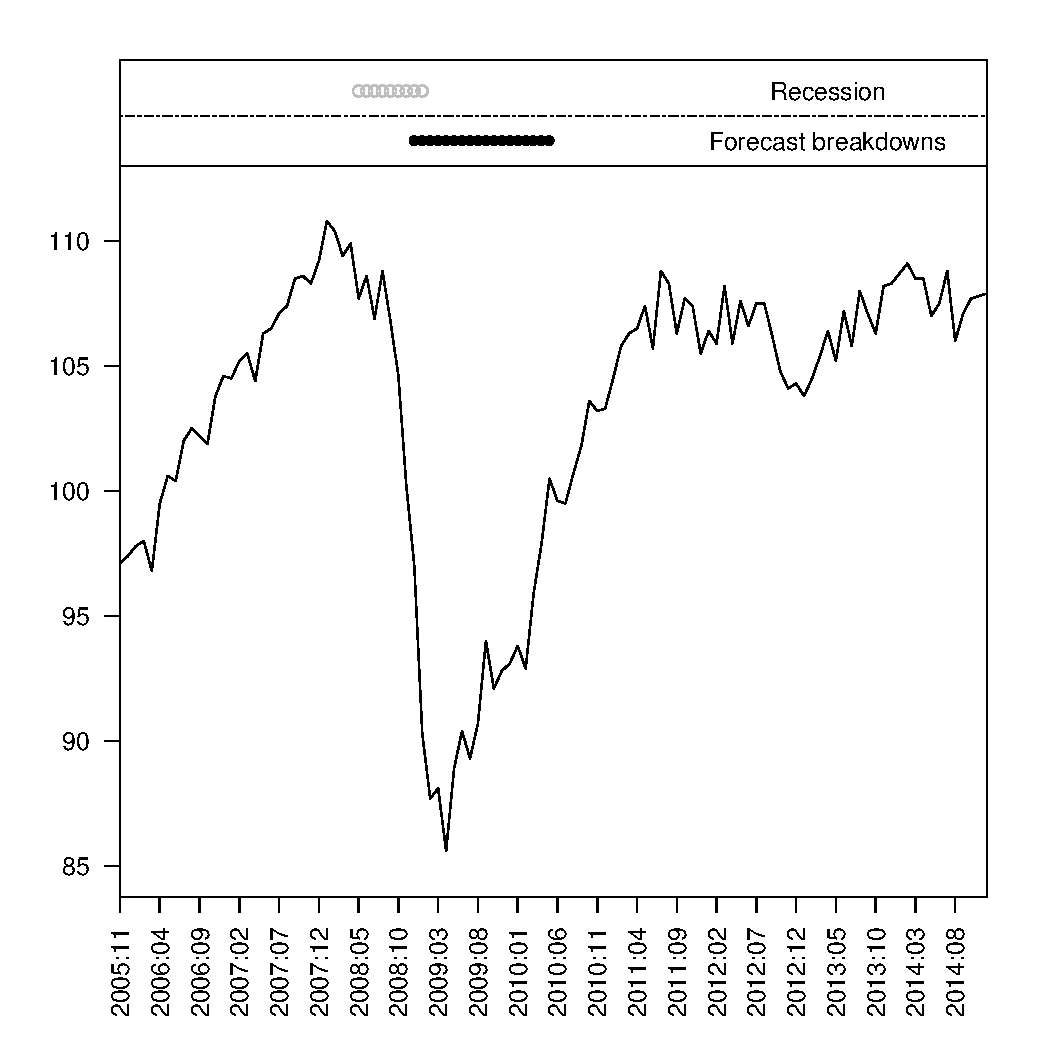
\includegraphics[scale=0.85]{ip_crisis_breakdowns}
\end{figure}

% % % % % % % % % % % % % % % % % % % % % % % % % % % % % % % % % % % % % % % % % % % % % % % % % %
\begin{figure}[htbp]
	\caption{Percentage of models included in MCS\label{fig:Percentage-of-models}}
	\begin{centering}
		\subfloat[All periods, 2005:12-2014:04\label{fig:All-periods, 2005:12-2014:04}]{
			\centering{}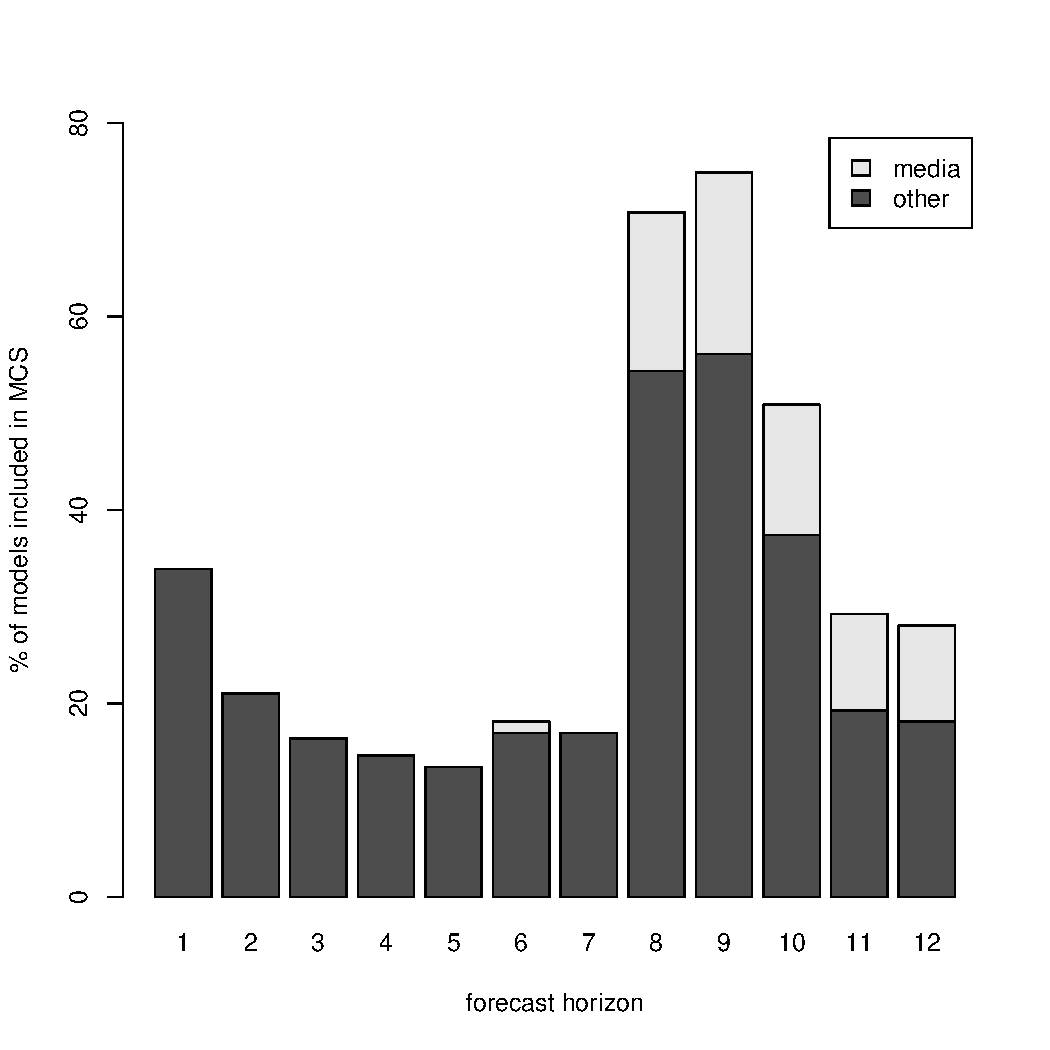
\includegraphics[scale=0.5]{mcs_share_media_all}}
		\par\end{centering}
	\centering %{}
	\subfloat[Unstable (forecast breakdown) period, 2008:12-2010:06]{
		\centering{}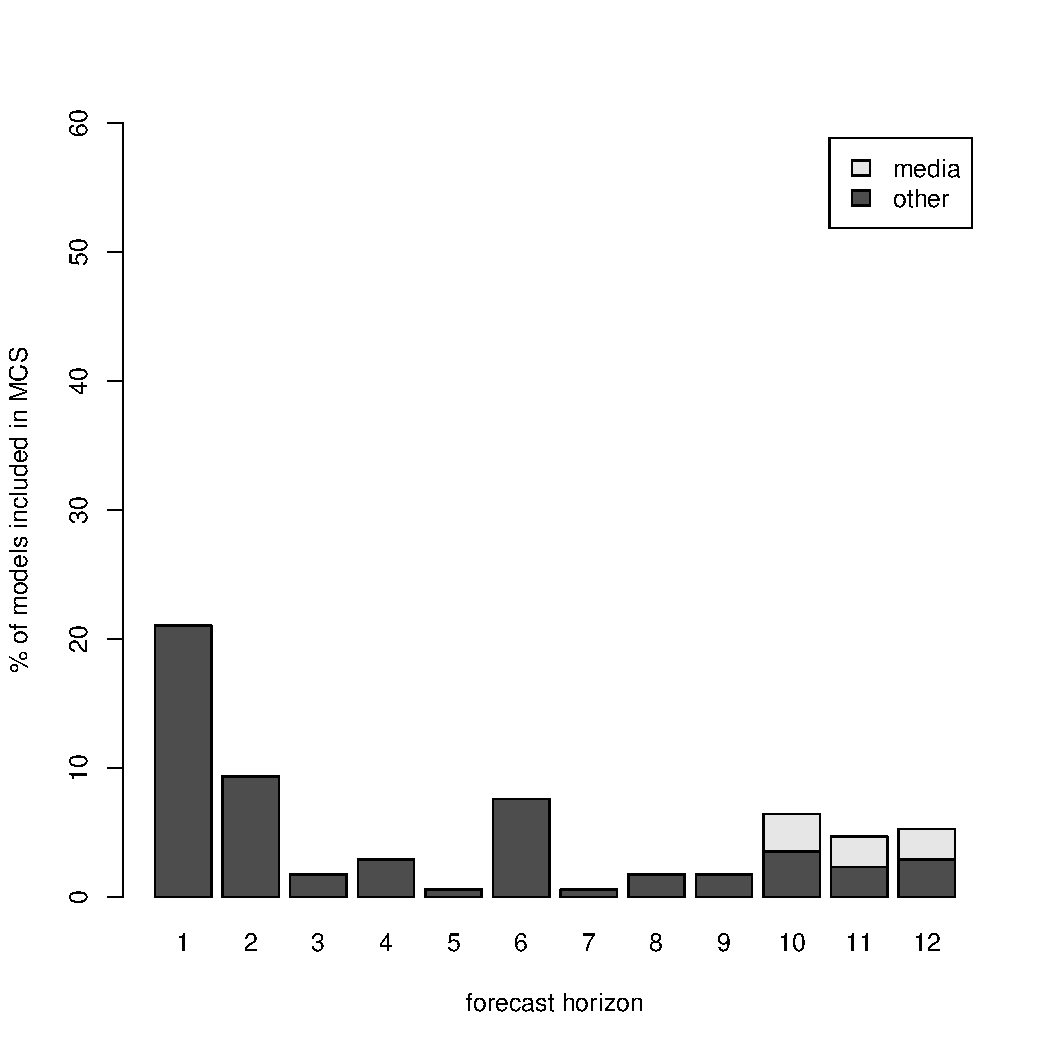
\includegraphics[scale=0.5]{mcs_share_media_recession}}
\end{figure}

\end{document}
